\documentclass[a4paper,10pt,hidelinks]{article}

\usepackage[margin=2cm]{geometry}

\usepackage{tikz}
\usepackage{hyperref}
\usepackage{algorithm}
\usepackage{algpseudocode}
\usepackage{amsmath}
\usepackage{amssymb}

\usepackage{listings}
\lstset{
	numbers=left,
	breaklines=true,
	tabsize=4
}

\newcommand{\algorithmautorefname}{Algorithm}

%opening
\title{Practical Assignment 2\\
Social Network Analysis}
\author{Bert Peters\\
s1147919}

\begin{document}

\maketitle

\section{Clustering Coefficient}

\begin{enumerate}
	\item A tree, by definition, has no loops, and therefore has a clustering coefficient of 0. Another example is a bipartite graph. This type of graph can only have cycles of at least length 4. This is because it is impossible for two edges in the same partition to have a connection. Cycles of length 4 do not contribute to the clustering coefficient, because that only counts the number of triangles, i.e. the number of cycles of length 3.

	\item There are several possible such graphs. One of them is shown in \autoref{fig:graph-no-clustering}.

	\item Contructing an unclustered graph is trivial for when $m \leq n$, because we can construct a circle graph of size $n$ and remove edges to arrive at the desired number of edges. The algorithm is shown in \autoref{algo:algo-no-clustering} and runs in $O(m)$.

		The algorithm works by adding repeatedly connecting each node $v_i$ to another node $v_{i + \delta}$. This delta is increased over iterations, and is given by $\delta = 3^s$ where $s$ is the current iteration number, starting at 1. This ensures that we do not create new loops shorter than 4, which is what we need in order to prevent clustering.
\end{enumerate}

\begin{figure}
	\centering
	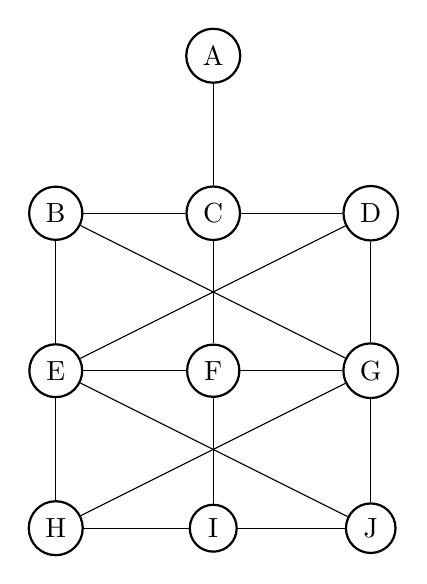
\begin{tikzpicture}[every node/.style={draw=black,thick,circle}]
		\node (A) at (0,4){A};
		\node (B) at (-2,2){B};
		\node (C) at (0,2){C};
		\node (D) at (2,2){D};
		\node (E) at (-2,0){E};
		\node (F) at (0,0){F};
		\node (G) at (2,0){G};
		\node (H) at (-2,-2){H};
		\node (I) at (0,-2){I};
		\node (J) at (2,-2){J};

		\draw (A) -- (C);
		\draw (B) -- (C);
		\draw (C) -- (D);
		\draw (B) -- (E);
		\draw (C) -- (F);
		\draw (E) -- (F);
		\draw (D) -- (G);
		\draw (F) -- (G);
		\draw (E) -- (H);
		\draw (H) -- (I);
		\draw (F) -- (I);
		\draw (I) -- (J);
		\draw (G) -- (J);

		\draw (B) -- (G);
		\draw (D) -- (E);

		\draw (E) -- (J);
		\draw (G) -- (H);

	\end{tikzpicture}
	\caption{An undirected graph with 10 nodes, 15 edges, and a clustering coefficient of 0.}
	\label{fig:graph-no-clustering}
\end{figure}

\begin{algorithm}
	\caption{Constructing a graph with no clustering.}
	\label{algo:algo-no-clustering}

	\begin{algorithmic}
		\State $E \gets \emptyset$
		\State $s \gets 1$
		\While{$|E| < m \land 3^s < n$}
		\For{$v_i \in V \land |E| < m$}
		\State $E \gets E \cup \{\{v_i, v_{i + 3^s \text{ mod } n} \}\}$
		\EndFor
		\State $s \gets s + 1$
		\EndWhile
	\end{algorithmic}

\end{algorithm}

\section{Densest Subgraph}

We start by computing the average degree and the current density. For a graph with a given $n, m$ this is easy, because the average degree is $\frac{2m}{n}$ and the density is half of that. We run our algortihm, by iteratively removing the nodes with a degree lower than the average degree from our $V$ and $E$, and repeat the process until we cannot delete nodes anymore.

Using the above algorithm, we arrive at the results as shown in \autoref{tab:densest-subgraph}. We see that after iteration 1, we already find our maximum, with a density of 1.5. After that, we still delete nodes twice, until we arrive at a graph with two nodes and cannot delete nodes any more.

\begin{table}
	\centering
	\begin{tabular}{r || l | r | r}
		Iteration & Subgraph & Density & Avg. degree\\
		\hline
		0   & $\{A B C D E F H I J K L\}$ & $\frac{16}{11} \approx 1.45 $ & $\frac{32}{11} \approx 2.9 $ \\
		1   & $\{A B E F J K\}$ & $ \frac{9}{6} = 1.5 $ & $ \frac{18}{6} = 3 $ \\
		2   & $\{B E F J\}$ & $\frac{5}{4} = 1.25$ & $\frac{10}{4} = 2.5$ \\
		3   & $\{E F\}$ & $\frac{1}{2} = 0.5$ & $\frac{2}{2} = 1$
	\end{tabular}
	\caption{Using the greedy algorithm to find the densest subgraph.}
	\label{tab:densest-subgraph}
\end{table}

\section{Twitter Network Extraction}

\subsection{Parsing the tweets}

We parse the tweets using a python script in \autoref{lst:preprocess}. It takes a list of files as arguments from the command line or data from the standard input. First, it splits the string twice on the first occurrence of a tab. It attempts to parse mentions out of a tweet using a regular expression. The expression used is a non-word character\footnote{A word character is defined as either an ascii letter character (upper case and lower case), a digit, or an underscore character (`\texttt{\_}'). Everything else, including the `\texttt{\^}' (start of string) and `\texttt{\$}' (end of string) metacharacters is considered a non-word character.}, followed by an `\texttt{@}', followed by $[1, 15]$ word characters\footnote{The specification of what is a valid twitter username can be found at \url{https://support.twitter.com/articles/101299}}, followed by by a non-word character. Requiring a non-word character before the mention filters out email addresses, which occur frequently in the dataset. The resulting usernames are put in lowercase, because twitter usernames are case-insensitive.

The script determines a mapping from usernames to integers, because this is more convenient to handle programmatically in the analysis. It outputs a Gephi-edgelist compatible list of mentions to the standard output, and a Gephi-nodelist compatible username mapping to the standard error.

There are still a number of things that the parser does wrong. The most prevalent error happens when users have no separator (either white space or punctuation) between a mention and the following text. In this case, it is impossible to determine where the username ends and the tweet continues. This can only be solved when you know all usernames in your dataset.

This problems described above can, however, be solved by using the twitter api. It provides any mentions included in a message as meta data, removing the need for complicated parsers. Implementing this is outside the scope of this assignment.

\subsection{Dataset statistics}

\begin{table}
	\centering
	\begin{tabular}{l || r | r | c | r | r | c | r}
		\multicolumn{1}{c ||}{Dataset} & \multicolumn{1}{c |}{$|V|$} & \multicolumn{1}{c |}{$|E|$} & $D$ & \multicolumn{1}{c |}{$|V_{giant}|$} & \multicolumn{1}{c |}{$|E_{giant}|$} & $D_{giant}$ & Diameter\\
		\hline
		\texttt{twitter-small} & 47568 & 53449 & $2.4 \cdot 10^{-5}$ & 32351 & 44135 & $4.2 \cdot 10^{-5}$ & 21 \\
		\texttt{twitter-larger} & 398388 & 691080 & $4.4 \cdot 10^{-6}$ & 328358 & 648832 & $6.0 \cdot 10^{-6}$ & 23 \\
		\texttt{twitter} & 8663906 & 57959449 & $7.7 \cdot  10^{-7}$ & 8402847 & 57813254 & $8.2 \cdot 10^{-7}$ & ?
	\end{tabular}
	\caption{Dataset statistics}
	\label{tab:dataset-stats}
\end{table}

We consider the graph as an undirected graph. We use our parser program to get some statistics about our dataset. The results are shown in \autoref{tab:dataset-stats}. For the degree distribution, we reuse the python script from the previous assignment. This gives us the distribution as shown in \autoref{fig:graph-no-clustering}.

Edges occurring multiple times are counted towards node degrees, but not towards the number of edges. In other words, the equation $\sum\limits_{v_i} k(v_i) = 2|V|$ does not hold.

For density, we take the measure $D = \frac{|V|}{|E|(|E| - 1)}$. Since, in a social network, the average degree does not depend on the number of nodes in the network, we we expect the density to drop linearly with the number of nodes. This is because $\lim_{n \rightarrow \infty} \frac{cn}{n (n - 1)} = \frac{1}{n}$. Furthermore, there should be a slightly lower  density in the entire network and that in the giant component. This is because the network contains a lot of isolated nodes, i.e. people that have tweeted, but not mentioned, and who have not been mentioned.

\begin{figure}
	\centering
	\includegraphics[scale=0.8]{degree-distributions.pdf}
	\caption{Degree distribution for all datasets.}
	\label{fig:degree-distributions}
\end{figure}

\begin{figure}
	\centering
	\includegraphics[scale=0.8]{distance-distribution}
	\caption{Approximate distance distributions for all datasets. Bars are relative within one dataset.}
	\label{fig:distance-distributions}
\end{figure}

It is infeasible to compute the exact distance distribution for all networks, as this requires computing $\frac{1}{2} n (n-1)$ distances. To do so would require $O(nm)$ time, to perform $n$ breadth first searches. Instead, we use an approximation. For this, we perform 100 breadth first searches and count how often each distance occurs. We then normalize by dividing by the total number of paths found, and arrive at the distribution as shown in \autoref{fig:distance-distributions}.

\subsection{Top Twitter users}
To compute the top 20 twitter users in our dataset, we consider the following centrality measures:

\begin{description}
	\item[Degree centrality] which is simply the degree of the node. For this experiment, we use the the out degree of a node for this. We then sort the nodes in descending order. We define it as $DC(u) = \max(\forall v \in V : k^\rightarrow(v))$.

	\item[Eccentricity centrality] which is the longest shortest path starting from a node. The idea is, that if your eccentricity is low, you are fairly central. It is defined as $EC(u) = \max(\forall v \in V : d(u, v))$.

	\item[Closeness centrality] which is somewhat related to the eccentricity centrality, but is slightly different, because we take the average path length rather than the total path length. This gives us $CC(u) = \frac{\sum_{v \neq u \in V}}{|V| - 1}$.
\end{description}

We then apply these measures to the \texttt{twitter-small} dataset. The results are shown in \autoref{tab:small-top-users}. For eccentricity, there are quite a few nodes with the same value.\footnote{This can be easily seen by observing that the $\forall u \in V: ecc(u) \leq \text{diameter}(G) \land ecc(u) \in \mathbb{N}$ by definition. This means that we do not have a lot of distinct values the eccentricity can take.} In this case, we use degree as a tie-breaker.

\begin{table}
	\centering
	\begin{tabular}{l || l | l | l}
		& \multicolumn{1}{c |}{$DC$} & \multicolumn{1}{c |}{$EC$} & \multicolumn{1}{c}{$CC$} \\
		\hline
		1 & theiphoneblog & mashable & theiphoneblog \\
		2 & ryanbarr & theiphoneblog & mashable\\
		3 & mashable & ryanbar & tweetmeme\\
		4 & scottbourne & scottbourne & iphone\_dev\\
		5 & scancafe & scancafe & tweetdeck\\
		6 & squarespace & squarespace & allthingsiphone \\
		7 & tweetmeme & tweetmeme & techcrunch \\
		8 & iphone\_dev & iphone\_dev & squarespace \\
		9 & tweetdeck & tweetdeck & kevinrose\\
		10 & kevinrose & kevinrose & randomslagathor \\
		11 & tomtom & techcrunch & musclenerd \\
		12 & techcrunch & engadget & engadget \\
		13 & patrickaltoft & iphoneincanada & scottbourne \\
		14 & iphoneincanada & tuaw & tuaw \\
		15 & quickpwn & guykawasaki & scancafe \\
		16 & engadget & musclenerd & iphoneincanada \\
		17 & tinteract &  chrispirillo & razorianfly \\
		18 & tuaw & parislemon & djsakebomb \\
		19 & guardiantech & trackle & reneritchie \\
		20 & igncom & johnbiggs & tmitechnews
	\end{tabular}
	\caption{Top 20 users in \texttt{twitter-small} according to different measures.}
	\label{tab:small-top-users}
\end{table}

We can not easily and objectively compare these rankings on quality, but we can numerically compare how different they are. We do this by counting inversions. This can be done in $O(l^2)$, with $l$ the number of items in our list. This is fairly doable for a top 20. Also, we have to account for nodes that are in one, but not in the other list. For this, we count it as an inversion against everything else, which means it has $l$ inversions.

When we take a look at the resulting top-users in \autoref{tab:small-top-users}, we can see that all three centrality measures are somewhat in agreement over the top users. This is not unexpected, as all three measures used for determining the rankings are somewhat correlated. For example, having a low eccentricity helps to get a lower closeness, and your closeness is very much influenced by your own outdegree.

\subsection{Community detection}
We attempt to detect the communities using Gephi. Ideally, we are looking for about 12 communities, as a lower amount would provide very little information and a higher amount would not be visually interprable. When setting the resolution to 1.0, we get thousands of communities. When we set it to 10.0, we find only 4 communities. Halfway in between at 5.0 we find 14 communities, which can be roughly interpreted as some subject on which users tweet.

\subsection{Visualisation}
To visualise the giant component of the \texttt{twitter-small} network, we use Gephi. Using the community detection described in the previous section, we color the nodes. Furthermore, we scale the nodes according to their betweenness centrality. The resulting network can be seen in \autoref{fig:visualisation}. While improving upon this visualisation, Gephi gave up, so I gave up on visualising.

\begin{figure}
	\centering
	\includegraphics[scale=0.8]{visualisation.pdf}
	\caption{Visualisation of the \texttt{twitter-small} network. Colors are according to communities, and node size is proportional to betweenness centrality.}
	\label{fig:visualisation}
\end{figure}

\subsection{Analysing the \texttt{twitter-larger} dataset}
\begin{table}
	\centering
	\begin{tabular}{l || l | l | l}
		& \multicolumn{1}{c |}{$DC$} & \multicolumn{1}{c |}{$EC$} & \multicolumn{1}{c}{$CC$} \\
		\hline
		1 & uberguineapig & uberguineapig & uberguineapig \\
		2 & mobil\_tipps & mobil\_tipps & mashable\\
		3 & dloblack & iphone\_mob & iphone\_mob \\
		4 & iphonedevnews & muenchner\_kindl & techcrunch \\
		5 & iphone\_nikki & iphone\_jedi & tweetmeme \\
		6 & macandiphone & maclounge & startonlinetwit \\
		7 & riggledo & botiphone & razorianfly \\
		8 & muenchner\_kindl & savvybanana & sebastianpage \\
		9 & danlaforce & ezf\_executives & tuaw \\
		10 & iphone\_jedi & kaisersoeze & muenchner\_kindl \\
		11 & tm\_iphone & tommytrc & dudeman718 \\
		12 & allthingsiphone & magicbaseball1 & tm\_iphone \\
		13 & inflight\_wifi & flipbooks & topiphone \\
		14 & ipodtouchroom & jwforson & krapps \\
		15 & esteves08 & the\_borg & mayhemstudios \\
		16 & supsappel & bildarchiv & kaisersoeze \\
		17 & iphone3gupdates & shellykramer & theiphoneblog \\
		18 & tramain360 & randomslagathor & bradgal \\
		19 & csrandom & appgirlreviews & scobleizer \\
		20 & locaconpistolas & earthxplorer & tm\_technology
	\end{tabular}
	\caption{Top 20 users in \texttt{twitter-larger} according to different measures.}
	\label{tab:larger-top-users}
\end{table}

Since we use our own parser (see appendices) we can quite easily run the statistics on the \texttt{twitter-larger} dataset. The results are incorporated in \autoref{tab:dataset-stats}, \autoref{fig:degree-distributions}, and \autoref{fig:distance-distributions}. Furthermore, we can compute the eccentricity for every node exactly using the algorithm by F.W. Takes et al. and arrive at the eccentricity for each node in approximately 17,000 breadth first searches. This is about 20 times faster than the naive approach.

The closeness centrality is a bit more challenging to compute. Instead, we approximate it by sampling the distance between 10,000 randomly selected nodes and everything else, and averaging those results.\footnote{While this method is a lot of work, it is doable in about an hour, while doing the entire computation would take slightly over a day.} As a slight bonus, calculating the eccentricities also gives us the diameter of the network, which is shown in \autoref{tab:dataset-stats}. What is interesting, is that the diameter of \texttt{twitter-larger} is only slightly greater than the diameter of \texttt{twitter-small}, despite the former being about ten times smaller than the latter. This is a property often observed in social networks.

\subsection{Bonus: Analysing the complete \texttt{twitter} dataset}
Our \texttt{C++} code is efficient enough to compute the dataset statistics in reasonable time while only needing 6 GiB of memory.\footnote{The system used had an Intel i7 CPU running at 3.4 GHz and 16 GiB of memory, but only a single thread and 6 GiB of memory was used.} The data is shown in \autoref{tab:dataset-stats}, \autoref{fig:degree-distributions}, and \autoref{fig:distance-distributions}. We used the same approximation of the distance distribution that we used for the other datasets, which took about 40 minutes to compute.

We can also still sample the network 

Computing all eccentricities however was more challenging. At the time of writing, we have spent over 21 hours of computation doing a total of 2,872 breadth first searches, with 1,302,102 eccentricities not yet known. This gives us an average of one BFS every 26 seconds. This, along with the observation that we find at least one eccentricity per search, gives us an upper bound of 391 days for the remaining computation. I therefore do not except a result to this. While I have observed a speed up of over 100 using the algorithm, I still do not expect to see a result before the deadline. Mostly because the system will be rebooted Sunday at 03:00, losing all my progress.

It could still be possible to compute the rankings, as the eccentricity bounds for most low eccentricity nodes become tight very quickly, and for other nodes the bounds are at least very close. Doing so is outside the scope of this project however.

\pagebreak

\appendix

\section{preprocess.py}
\label{lst:preprocess}
\lstinputlisting[language=python]{preprocess.py}
\pagebreak

\section{Makefile}
\lstinputlisting[language=make]{Makefile}
\pagebreak

\section{parser.cpp}

\lstinputlisting[language=c++]{parser.cpp}

\pagebreak

\section{TwitterGraph.hpp}

\lstinputlisting[language=c++]{TwitterGraph.hpp}

\pagebreak

\section{TwitterGraph.cpp}

\lstinputlisting[language=c++]{TwitterGraph.cpp}

\pagebreak

\section{eccentricity.cpp}
This file contains the method used to compute the eccentricity of all nodes and the diameter of the network. It is adapted from the presentation \emph{Determining the Diameter of Small World Networks} by F.W. Takes and W.A. Kosters. The original presentation containing the algorithm can be found at \url{http://liacs.leidenuniv.nl/~takesfw/SNACS/diameter.pdf}.

\lstinputlisting[language=c++]{eccentricity.cpp}

\pagebreak

\section{closeness.cpp}

This file contains the method used to approximate the closeness of a particular node.

\lstinputlisting[language=c++]{closeness.cpp}
\end{document}
